\documentclass[11pt,a4paper]{article}

\usepackage[utf8]{inputenc}
\usepackage{lmodern}
\usepackage[T1]{fontenc}
\usepackage[spanish,es-noquoting,es-tabla]{babel}
\usepackage[margin=2.3cm]{geometry}
\usepackage{graphicx}
\usepackage{array}
\usepackage{booktabs}
\usepackage{amsmath}
\usepackage{tikz}
\usetikzlibrary{arrows.meta,positioning}
\usepackage[font=small,labelfont=bf]{caption}
\usepackage[hidelinks]{hyperref}

\tikzset{
  caja/.style={draw, rounded corners=1.5pt, align=center,
               font=\scriptsize, inner sep=3.5pt, minimum height=10mm},
  flecha/.style={-{Stealth[length=2mm]}, semithick},
}

\newcolumntype{L}[1]{>{\raggedright\arraybackslash}p{#1}}

\setlength{\parindent}{0pt}
\setlength{\parskip}{5pt}
\renewcommand{\arraystretch}{1.25}

\title{\vspace{-1.5cm}\textbf{Replicación de \emph{Feature Visualization}}\\[3pt]
\large Los ResNet de Pl@ntNet-300K y una herramienta para inspeccionarlos}
\author{David Fernández Fernández y Javier Santamaría Pascual}
\date{}

\begin{document}
\maketitle

\section{Introducción}

Replicamos \emph{Feature Visualization}, de Olah, Mordvintsev y Schubert
(2017), sobre los ResNet preentrenados en Pl@ntNet-300K --el de 18 capas
como modelo de referencia, y los de 50 y 152 para comprobar que las
técnicas no dependen de la arquitectura--, y construimos encima una
herramienta de inspección: se le da una foto de una planta y responde qué
especie ve el modelo, qué neuronas enciende esa foto, en qué zona las
enciende y qué patrón busca cada una de ellas.

El artículo no publica ninguna métrica. Es un trabajo cualitativo: su
resultado son figuras, no cifras, de modo que no hay un número que igualar.
Lo que se replica son sus \textbf{técnicas} y sus \textbf{figuras}, y lo que
sí admite medida es el argumento que defiende, que sí es comprobable
(sección~\ref{sec:resultados}).

\begin{table}[htb]
\centering\small
\caption{Alcance de la replicación.}
\begin{tabular}{L{8.1cm} c L{5.1cm}}
\toprule
\textbf{Técnica del artículo} & \textbf{Repr.} & \textbf{Dónde} \\
\midrule
Objetivos: Neuron, Channel, Layer/DeepDream, Class Logits, Class
Probability & sí & \texttt{objetivos.py} \\
Direction, suma de neuronas, interpolación & sí & «Interaction between
Neurons» \\
Diversity & sí & \texttt{generar\_diversas()} \\
\emph{Preconditioning}: Fourier con color decorrelado & sí & contrastado
contra \texttt{lucid} \\
\emph{Transformation robustness} & sí & valores de la nota 9 del artículo \\
Penalización de frecuencia: L1, variación total, desenfoque & sí & fórmulas
de \texttt{lucid} \\
\emph{Dataset examples} & sí & \texttt{ejemplos\_del\_dataset()} \\
\emph{Learned priors} (GAN/VAE) & \textbf{no} & fuera de alcance: exige
entrenar un generativo \\
\bottomrule
\end{tabular}
\end{table}

\section{El artículo en resumen}

Una red entrenada es un montón de números y no dice qué ha aprendido. La
visualización de características lo plantea al revés: en lugar de preguntar
qué responde la red ante una foto, busca \textbf{qué imagen haría responder
al máximo} a una unidad concreta. Se parte de ruido y se asciende por el
gradiente hasta que esa unidad se activa todo lo posible.

El punto clave, y lo que distingue esta técnica del entrenamiento, es que
\textbf{los pesos del modelo no se tocan}. Se cargan congelados, y lo único
que recibe gradiente —y por tanto lo único que se optimiza— es la imagen de
entrada.

Hecho así de ingenuo el método no funciona: produce ruido adversarial, una
imagen que activa muchísimo la unidad y no se parece a nada reconocible. El
artículo sostiene que la diferencia entre ruido y patrón interpretable está
en la regularización, y describe tres familias: penalizaciones de frecuencia
sobre la imagen, robustez a transformaciones, y \emph{learned priors}.
Reproducimos las dos primeras.

\subsection{Qué se puede maximizar}

\begin{table}[htb]
\centering\small
\caption{Los ocho objetivos implementados. Los cinco primeros son los de
«Optimization Objectives»; los tres últimos, los de «The Interaction between
Neurons».}
\begin{tabular}{l l L{7.6cm}}
\toprule
\textbf{Tipo} & \textbf{Expresión} & \textbf{Qué maximiza} \\
\midrule
\texttt{canal} & \texttt{layer\_n[:,:,z]} & la media espacial de un canal;
es el valor por defecto \\
\texttt{neurona} & \texttt{layer\_n[x,y,z]} & una sola posición de ese canal \\
\texttt{capa} & \texttt{layer\_n[:,:,:]\textsuperscript{2}} & la capa
entera: es DeepDream, e ignora el canal \\
\texttt{logit} & \texttt{pre\_softmax[k]} & la puntuación de una clase \\
\texttt{probabilidad} & \texttt{softmax[k]} & esa clase, hundiendo además
las demás \\
\texttt{direccion} & \texttt{v $\cdot$ layer\_n[x,y,:]} & una combinación de
canales, no uno solo \\
\texttt{suma} & varios canales a la vez & el objetivo \emph{jointly
optimized} \\
\texttt{interpolacion} & de un canal a otro & la transición entre dos
unidades \\
\bottomrule
\end{tabular}
\end{table}

\section{Arquitectura y funcionamiento}

El sistema tiene dos mitades que no se mezclan. La de replicación contiene
los objetivos, el bucle de optimización y la fachada; la del aplicativo es
una interfaz web que solo carga un \emph{checkpoint} y responde. El
aplicativo no importa nada del código de entrenamiento: habla únicamente con
la fachada, que es el contrato.

\subsection{Los modelos}

Pl@ntNet-300K publica tres \emph{checkpoints} y el sistema admite los tres,
sobre las mismas 1081 especies. Cambiar de uno a otro es cambiar dos claves
del fichero de configuración: no hay código específico de ninguna
arquitectura, y las cuatro capas que ofrece la interfaz
(\texttt{layer1.1.conv2} a \texttt{layer4.1.conv2}) existen en los tres.

\begin{center}\small
\begin{tabular}{l r l}
\toprule
\textbf{Arquitectura} & \textbf{Parámetros} & \textbf{Papel en el trabajo} \\
\midrule
ResNet-18 & 11\,731\,065 & El de referencia. Todas las cifras y figuras de
este informe salen de él. \\
ResNet-50 & 25\,723\,001 & Mismas técnicas, unidades más anchas. \\
ResNet-152 & 60\,358\,777 & El más profundo de los tres. \\
\bottomrule
\end{tabular}
\end{center}

Que las técnicas no dependan de la arquitectura es, precisamente, parte de
lo que el artículo sostiene: lo que describe son métodos para interrogar
una red convolucional cualquiera, no recetas atadas a un modelo concreto.
Poder ejecutarlos sobre tres redes de tamaño muy distinto es la forma de
comprobarlo.

\subsection{El recorrido de la aplicación}

\begin{figure}[htb]
\centering
\begin{tikzpicture}[node distance=5.5mm]
\node[caja] (a) {Foto\\de entrada};
\node[caja, right=of a] (b) {\textbf{Predicción}\\\texttt{predecir()}\\qué
especie es};
\node[caja, right=of b] (c) {\textbf{Ranking}\\\texttt{listar\_neuronas()}\\qué
canales enciende};
\node[caja, right=of c] (d) {\textbf{Mapa}\\\texttt{mapa\_activacion()}\\dónde
los enciende};
\node[caja, right=of d] (e) {\textbf{Optimización}\\\texttt{generar\_imagen()}\\qué
patrón busca};
\draw[flecha] (a) -- (b); \draw[flecha] (b) -- (c);
\draw[flecha] (c) -- (d); \draw[flecha] (d) -- (e);
\end{tikzpicture}
\caption{Las cuatro etapas. Son las mismas desde la interfaz web y desde la
API en Python, porque ambas llaman a las mismas funciones de la fachada.}
\label{fig:recorrido}
\end{figure}

Las etapas 2 y 3 son el mismo cálculo visto de dos maneras, y conviene
entender por qué. Un \emph{hook} captura la salida de la capa elegida, que
no es un número por canal sino una rejilla: $56\times56$ en
\texttt{layer1.1.conv2}, $28\times28$ en \texttt{layer2}, $14\times14$ en
\texttt{layer3} y $7\times7$ en \texttt{layer4}. El ranking promedia esa
rejilla para poder ordenar los canales —ese promedio es exactamente el
objetivo \emph{Channel} del artículo, medido en lugar de maximizado— y el
mapa de activación devuelve la misma rejilla \textbf{antes} del promedio,
reescalada al tamaño de la foto. El mapa es, por tanto, el eslabón que
conecta un número del ranking con una zona concreta de la imagen.

\subsection{El bucle de optimización}

\begin{figure}[htb]
\centering
\begin{tikzpicture}[node distance=5mm]
\node[caja] (p) {Parámetros\\de la imagen};
\node[caja, right=of p] (q) {\textbf{Parametrización}\\espectro de
Fourier,\\color decorrelado};
\node[caja, right=of q] (r) {\textbf{Robustez}\\relleno, jitter,\\escala,
rotación};
\node[caja, right=of r] (s) {Normalización\\y modelo\\\textbf{congelado}};
\node[caja, below=7mm of s] (t) {\textbf{Objetivo}\\el escalar a\\maximizar};
\node[caja, left=of t] (u) {\textbf{Pérdida}\\$-$activación\\$+$
penalizadores};
\node[caja, left=of u] (v) {\texttt{backward()}\\y paso de Adam};
\draw[flecha] (p) -- (q); \draw[flecha] (q) -- (r); \draw[flecha] (r) -- (s);
\draw[flecha] (s) -- (t); \draw[flecha] (t) -- (u); \draw[flecha] (u) -- (v);
\draw[flecha] (v) -| (p);
\end{tikzpicture}
\caption{Una iteración. El gradiente llega hasta los parámetros de la
imagen y Adam los actualiza; los pesos del modelo quedan intactos.}
\label{fig:bucle}
\end{figure}

Dos piezas de la figura~\ref{fig:bucle} son las que el artículo defiende y
las que marcan la diferencia entre un patrón y ruido. La
\textbf{parametrización} no optimiza los píxeles directamente, sino un
espectro de Fourier escalado por $1/f^{\,\text{decay}}$ con decorrelación de
color y una sigmoide: es el \emph{preconditioning}, y lo que hace es cambiar
qué direcciones del espacio de imágenes son «baratas» para el optimizador.
La \textbf{robustez} encadena relleno, desplazamiento aleatorio, escalado,
rotación, un segundo desplazamiento y recorte, de modo que solo sobreviven
los patrones que activan la unidad aunque la imagen se mueva.

Si en los primeros pasos el gradiente es exactamente cero, se lanza la
excepción \texttt{UnidadMuerta}. Es el caso de una unidad ReLU muerta: no da
error por sí sola, simplemente devolvería el ruido inicial sin avisar de
nada.

\subsection{Configuración por capas}

\begin{figure}[htb]
\centering
\begin{tikzpicture}[node distance=9mm]
\node[caja] (a) {\texttt{configs/feature\_viz.yaml}\\todos los
hiperparámetros};
\node[caja, right=of a] (b) {Argumentos de la orden\\o controles de la
interfaz};
\node[caja, right=of b] (c) {Configuración\\resuelta};
\draw[flecha] (a) -- (b); \draw[flecha] (b) -- (c);
\end{tikzpicture}
\caption{Ningún hiperparámetro está escrito a fuego. Lo que se pasa por
fuera sobrescribe la clave correspondiente sin modificar el fichero, así que
el estado por defecto siempre es el documentado.}
\label{fig:config}
\end{figure}

El fichero se reparte en bloques para el objetivo, la imagen, la
optimización, la regularización, la robustez, la normalización, la salida y
el registro de experimentos. La interfaz expone nueve de esos parámetros
como controles —los pasos de optimización, los tres penalizadores de
frecuencia, el desplazamiento, la rotación, la escala y los dos
interruptores que apagan la robustez y el espacio de Fourier—, que son
precisamente los de las figuras interactivas del artículo. A ellos se suman
el selector de capa y el de objetivo.

Los dos interruptores son los que mejor ilustran el argumento central: al
apagarlos la activación final sube y la imagen deja de parecerse a nada.

\subsection{Organización del repositorio}

\begin{table}[htb]
\centering\small
\caption{Qué hay en cada sitio.}
\begin{tabular}{l L{10.8cm}}
\toprule
\textbf{Carpeta o archivo} & \textbf{Responsabilidad} \\
\midrule
\texttt{src/interpretability/objetivos.py} & Qué se maximiza: los ocho
objetivos del artículo. \\
\texttt{src/interpretability/feature\_viz.py} & El bucle, la parametrización
y la robustez. También es la orden de consola. \\
\texttt{src/interpretability/api.py} & La fachada: el único contrato que
consume el aplicativo. \\
\texttt{src/app/serve.py} & La interfaz web. No importa nada de
\texttt{src/training/}. \\
\texttt{src/utils/} & Semillas, registro de experimentos y utilidades. \\
\texttt{configs/} & Todos los hiperparámetros. \\
\texttt{scripts/} & Descarga de datos y pesos, medida del acierto y las dos
demostraciones. \\
\texttt{tests/} & 133 pruebas de forma, invariancia y reproducibilidad. \\
\bottomrule
\end{tabular}
\end{table}

Las semillas se fijan en un único módulo y las dependencias van con versión
exacta; entre ejecuciones distintas la activación final puede variar en
torno a un 1\,\%. Las pruebas no dependen de los pesos: usan un ResNet-18
sin entrenar, porque los \texttt{.tar} no se versionan. Cada ejecución queda
registrada en Weights \& Biases con la activación, la pérdida, la aspereza
de la imagen y la imagen en curso cada 32 pasos, que es la figura
\emph{Step 1 / 32 / 128 / 256} del artículo generada automáticamente.

\section{Resultados}
\label{sec:resultados}

\begin{figure}[htb]
\centering
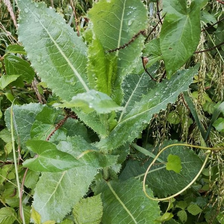
\includegraphics[width=0.3\linewidth]{figuras/foto.png}\hspace{4mm}
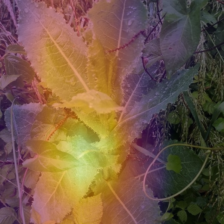
\includegraphics[width=0.3\linewidth]{figuras/mapa.png}\hspace{4mm}
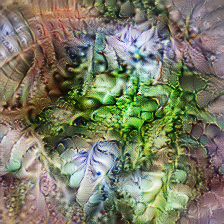
\includegraphics[width=0.3\linewidth]{figuras/patron.png}
\caption{El recorrido completo sobre una misma foto. Izquierda: la entrada,
clasificada como \emph{Lactuca serriola} con un 63,0\,\% de probabilidad.
Centro: el mapa de activación del canal 362 de \texttt{layer4.1.conv2}, el
más activo de esa capa ($+0{,}3392$). Derecha: la imagen optimizada desde
ruido para maximizar ese mismo canal.}
\label{fig:pipeline}
\end{figure}

\subsection{Verificación del \emph{checkpoint}}

Antes de interpretar un modelo hay que asegurarse de que se está
interpretando el modelo correcto, y ese riesgo aquí es real: un error en la
normalización de entrada o en el mapa de clases \textbf{no produce ningún
fallo visible}. El programa sigue funcionando y las visualizaciones salen
igual de vistosas, solo que entonces son de otra unidad, o de un modelo mal
cargado, y todo lo que se concluya de ellas es falso. Medir el acierto es
la forma de detectarlo, porque se desploma en cuanto algo de eso está mal.

Sobre 120 fotos del \emph{split} de test, una por especie, entre las 144
especies con 300 o más imágenes de entrenamiento, el clasificador acierta
\textbf{80,0\% de top-1 y 95,0\% de top-5}. Son cifras coherentes con un
ResNet-18 sobre 1081 clases, de modo que el \emph{checkpoint} se está
cargando y usando como debe y las visualizaciones son de lo que decimos.

La misma medida resolvió además una ambigüedad que el \emph{checkpoint} no
documenta: con qué estadísticas se normalizó. Las de ImageNet dan 80,0\% y
las de Pl@ntNet-300K 79,2\%, con el top-5 idéntico. Una imagen de
diferencia en 120, así que la elección no cambia el resultado y deja de ser
una duda abierta.

\subsection{El argumento central, cuantificado}

El artículo sostiene que sin robustez a transformaciones la optimización
alcanza un óptimo mejor y una imagen peor. Es lo único verdaderamente
medible de la replicación, y se comprueba desactivándola.

% Sin flotar y dentro de un minipage: esta tabla es el dato que sostiene el
% parrafo siguiente. Si flota se lleva la evidencia detras de la conclusion,
% y sin el minipage el pie se queda huerfano al final de la pagina.
\begin{center}
\begin{minipage}{\linewidth}
\captionof{table}{Ablación de la robustez. Canal 181 de
\texttt{layer3.1.conv2}, 256 pasos. La aspereza es la variación total de la
imagen, que mide cuánto se parece a ruido: cuanto más alta, peor.}
\vspace{2pt}
\centering\small
\begin{tabular}{l c c}
\toprule
 & \textbf{Activación final} & \textbf{Aspereza} \\
\midrule
Con robustez & $+4{,}93$ & $0{,}164$ \\
Sin robustez & $+7{,}15$ & $0{,}245$ \\
\midrule
Diferencia & +45\% & +49\% \\
\bottomrule
\end{tabular}
\end{minipage}
\end{center}

La activación sube un 45\,\% mientras la imagen empeora un 49\,\%. Mejor
óptimo, peor imagen: exactamente lo que el artículo defiende. Apagar el
espacio de Fourier produce el mismo efecto, con convergencia a ruido
adversarial.

\section{Diferencias con el artículo original}

\begin{table}[htb]
\centering\small
\begin{tabular}{L{4.6cm} L{4.6cm} L{5.6cm}}
\toprule
\textbf{Artículo original} & \textbf{Nuestro proyecto} & \textbf{Motivo} \\
\midrule
GoogLeNet entrenada en ImageNet. & Los tres ResNet de Pl@ntNet-300K (18, 50
y 152 capas), 1081 especies. & Es el dominio de la asignatura. Ejecutar las
mismas técnicas sobre tres redes de tamaño muy distinto comprueba que no
dependen de la arquitectura. \\
2560 pasos de optimización por figura. & 256 por defecto, ajustable entre
32 y 1024 desde la interfaz, y sin límite desde el fichero de
configuración. & Coste por imagen. Con 256 las figuras salen algo menos
refinadas; subir ese único parámetro a 2560 recupera la fidelidad del
artículo sin tocar una línea de código. \\
Valores de robustez de la nota al pie 9. & Los mismos de la nota al pie 9.
& Para una replicación manda el artículo. \texttt{lucid}, su propia
biblioteca, usa otros valores en \texttt{standard\_transforms}. \\
Coeficientes L1 $-0{,}05$, TV $-0{,}25$, desenfoque $-1$. & No se copian
literalmente. & Allí los términos se \textbf{suman} sobre 150\,528 elementos
y aquí se \textbf{promedian}; además allí se maximiza y se restan, y aquí se
minimiza y se suman. \\
Tres familias de regularización, \emph{learned priors} incluidos. & Las dos
primeras. & Los \emph{learned priors} exigen entrenar un modelo generativo,
que es un proyecto aparte. \\
\bottomrule
\end{tabular}
\end{table}

\begin{thebibliography}{9}\small
\bibitem{olah2017} C.~Olah, A.~Mordvintsev y L.~Schubert.
\emph{Feature Visualization}. Distill, 2017. DOI: 10.23915/distill.00007.
\bibitem{plantnet} C.~Garcin, A.~Joly, P.~Bonnet et al.
\emph{Pl@ntNet-300K: a plant image dataset with high label ambiguity and a
long-tailed distribution}. NeurIPS Datasets and Benchmarks, 2021.
\bibitem{lucid} \emph{tensorflow/lucid}. Implementación de referencia del
artículo, en TensorFlow.
\end{thebibliography}

\end{document}
